\documentclass[11pt,oneside]{article}
\usepackage[T1]{fontenc}
\usepackage[utf8]{inputenc}
%\DeclareUnicodeCharacter{00A0}{ }
\usepackage[adobe-utopia]{mathdesign}

\usepackage{amsmath}
\usepackage[francais]{babel}
\usepackage[dvips]{graphicx}
%\usepackage{here}
\usepackage{framed}
\usepackage[normalem]{ulem}
\usepackage{fancyhdr}
\usepackage{titlesec}
\usepackage{vmargin}

\usepackage{amsmath}
\usepackage{ifthen}
\usepackage{multirow}
\usepackage{multicol} % Portions de texte en colonnes

%\usepackage{xltxtra} % Logo XeLaTeX
%\usepackage{pst-solides3d}
\usepackage{color}
%\usepackage{colortbl}
\usepackage{titletoc} % Pour la mise en forme de la table des matières

%\usepackage[crop=off]{auto-pst-pdf}
%\usepackage{bclogo}


%\usepackage{longtable}
%\usepackage{flafter}%floatants après la référence
%\usepackage{pst-solides3d}
%\usepackage{pstricks}
%\usepackage{minitoc}
%\setcounter{minitocdepth}{4}
%\usepackage{draftcopy}% "Brouillon"
%\usepackage{floatflt}
%\usepackage{psfrag}
%\usepackage{listings} % Permet d'insérer du code de programmation
%\usepackage{lmodern}
%\usepackage[adobe-utopia,uppercase=upright,greeklowercase=upright]{mathdesign}
%\usepackage{minionpro}
%\usepackage{pifont}
%\usepackage{amssymb}
%\usepackage[francais]{varioref}

\setmarginsrb{1.5cm}{1cm}{1cm}{1.5cm}{1cm}{1cm}{1cm}{1cm}

\definecolor{gris25}{gray}{0.75}
\definecolor{bleu}{RGB}{18,33,98}
\definecolor{bleuf}{RGB}{42,94,171}
\definecolor{bleuc}{RGB}{231,239,247}
\definecolor{rougef}{RGB}{185,18,27}
\definecolor{rougec}{RGB}{255,230,231}
\definecolor{vertf}{RGB}{103,126,82}
\definecolor{vertc}{RGB}{220,255,191}
\definecolor{violetf}{RGB}{112,48,160}
\definecolor{violetc}{RGB}{230,224,236}
\definecolor{jaunec}{RGB}{220,255,191}

\usepackage{style/schemabloc}
%Si le boolen xp est vrai : compilation pour xabi
%Sinon compilation Damien
\newboolean{xp}
\setboolean{xp}{true}

\newboolean{prof}
\setboolean{prof}{true}

\def\xxtitre{\ifthenelse{\boolean{xp}}{
CI 2 -- SLCI : Étude du comportement des Systèmes Linéaires Continus Invariants}{
}}

\def\xxsoustitre{\ifthenelse{\boolean{xp}}{
Exercice de colle}{
}}


\def\xxauteur{\ifthenelse{\boolean{xp}}{
\noindent 2013 -- 2014 \\
Xavier \textsc{Pessoles}}{
}}


\def\xxpied{\ifthenelse{\boolean{xp}}{
CI 2 : SLCI\\
Exercice de colle \ifthenelse{\boolean{prof}}{P}{E}%
}{
}}

\usepackage[%
    pdftitle={SLCI - Systèmes du second ordre},
    pdfauthor={Xavier Pessoles},
    colorlinks=true,
    linkcolor=blue,
    citecolor=magenta]{hyperref}



\usepackage{pifont}
\sloppy
\hyphenpenalty 10000


\begin{document}






% \makeatletter \let\ps@plain\ps@empty \makeatother
%% DEBUT DU DOCUMENT
%% =================




%------------- En tetes et Pieds de Pages ------------


\pagestyle{fancy}
\ifthenelse{\boolean{xp}}{%
\renewcommand{\headrulewidth}{0pt}}{%
\renewcommand{\headrulewidth}{0.2pt}} %pour mettre le trait en haut
%\renewcommand{\headrulewidth}{0.2pt}

\fancyhead{}
\fancyhead[L]{%
\ifthenelse{\boolean{xp}}{%
\noindent\begin{minipage}[c]{2.6cm}%

\includegraphics[width=2cm]{png/logo_ptsi.png}%
\end{minipage}%
}{%
\footnotesize{\textit{\textsf{Lycée François Premier}}}
}}

\ifthenelse{\boolean{xp}}{%
\fancyhead[C]{\rule{12cm}{.5pt}}}{
}


\fancyhead[R]{%
\noindent\begin{minipage}[c]{3cm}
\begin{flushright}
\footnotesize{\textit{\textsf{Sciences Industrielles \\ de l'ingénieur}}}%
\end{flushright}
\end{minipage}
}


\ifthenelse{\boolean{xp}}{%
\fancyhead[C]{\rule{12cm}{.5pt}}}{
}

\renewcommand{\footrulewidth}{0.2pt}

\fancyfoot[C]{\footnotesize{\bfseries \thepage}}
\fancyfoot[L]{%
\begin{minipage}[c]{.2\linewidth}
\noindent\footnotesize{{\xxauteur}}
\end{minipage}
\ifthenelse{\boolean{xp}}{}{%
\begin{minipage}[c]{.15\linewidth}

\includegraphics[width=2cm]{png/logoCC.png}
\end{minipage}}
}


\fancyfoot[R]{\footnotesize{\xxpied}}



\begin{center}
 \Large\textsc{\xxtitre}
\end{center}

\begin{center}
 \large\textsc{\xxsoustitre}
\end{center}

%\vspace{.5cm}

\begin{center}
 \large\textsc{Correcteur de phare}
\end{center}

%\begin{flushright}
%\textit{D'après ressources d'Alain Caignot.}
%\end{flushright}




\subsection*{Cours}
\begin{itemize}
\item Donner la fonction de transfert d'un système du second ordre
\item Donner l'expression de la pseudo-période
\item Donner l'expression du dépassement
\item Donner l'allure de la réponse indicielle en fonction de la valeur du
coefficient d'amortissement
\end{itemize}


\section*{Correcteur de phare}


\textit{(Selon le concours CCP PSI 2003)}
\subsection*{Présentation du système}

L‘assiette d‘un véhicule se modifie avec sa charge, le profil de la route ou les
conditions de conduite (phase de freinage ou d‘accélération). Cette modification
entraîne une variation d‘inclinaison de l‘axe du faisceau lumineux produit par
les phares du véhicule. Ceux ci peuvent alors éblouir d‘autres conducteurs ou
mal éclairer la chaussée.


\begin{center}
 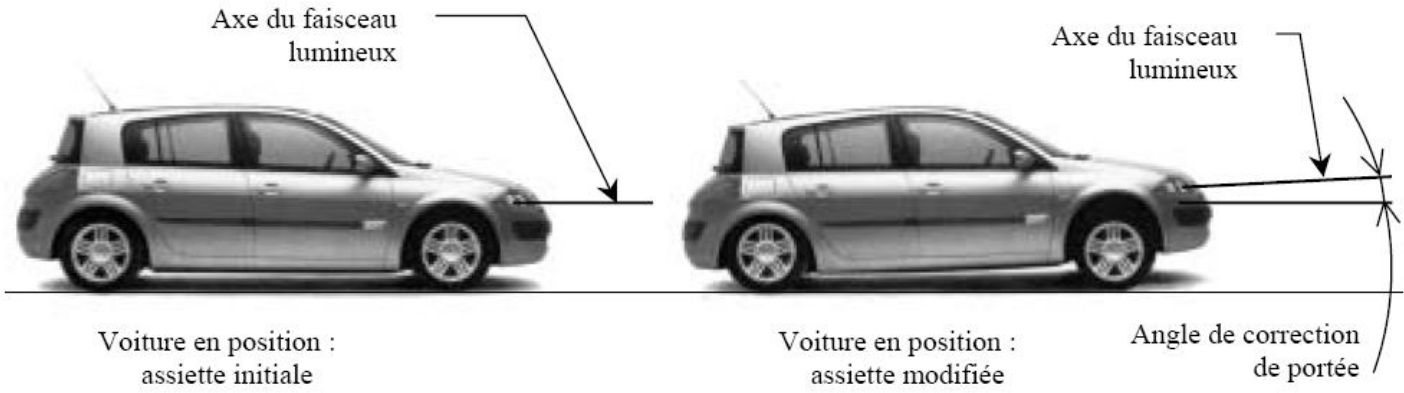
\includegraphics[width=.6\textwidth]{png/image1}
\end{center}
     
         Certaines voitures sont équipées de système de correction de portée. Ce
système fait appel à
des capteurs d‘assiette reliés aux essieux avant et arrière du véhicule. Les
données sont traitées
électroniquement par un calculateur et transmises aux actionneurs situés
derrière les projecteurs. La
position du projecteur est ajustée en maintenant un angle de faisceau optimal
évitant tout
éblouissement et fournissant le meilleur éclairage de la route.
Le système étudié est un correcteur de portée statique, qui corrige la portée
lorsque le véhicule est à
l‘arrêt et conserve cette correction lorsque le véhicule roule (le correcteur ne
tient compte que de la
variation d‘assiette due à la charge).

       Le but de l‘étude est d‘analyser le système et de montrer s‘il est
capable de corriger la portée
de manière dynamique, c‘est à dire en tenant compte des variations d‘assiette
dues au profil de la
route.

\subsubsection*{Éléments constitutifs du correcteur de portée}

\textbf{Capteurs d’assiette} : codeurs optiques permettant de mesurer le
débattement des suspensions.

\textbf{Système d’orientation : bloc d’orientation + moto-réducteur + système
vis écrou}

Le bloc d‘orientation supporte les différentes lampes du phare (codes,
clignotants...). Il peut pivoter
par rapport au support lié à la carrosserie autour d‘un axe horizontal (axe de
rotation indiqué sur la
figure ci-dessous). Le bloc est protégé par une vitre liée à la carrosserie. Ce
mouvement est motorisé
grâce au moto-réducteur + système vis écrou. Il existe aussi une possibilité de
réglage manuel en
sortie d‘usine ou en cas de défaillance du système électrique.

\begin{center}
 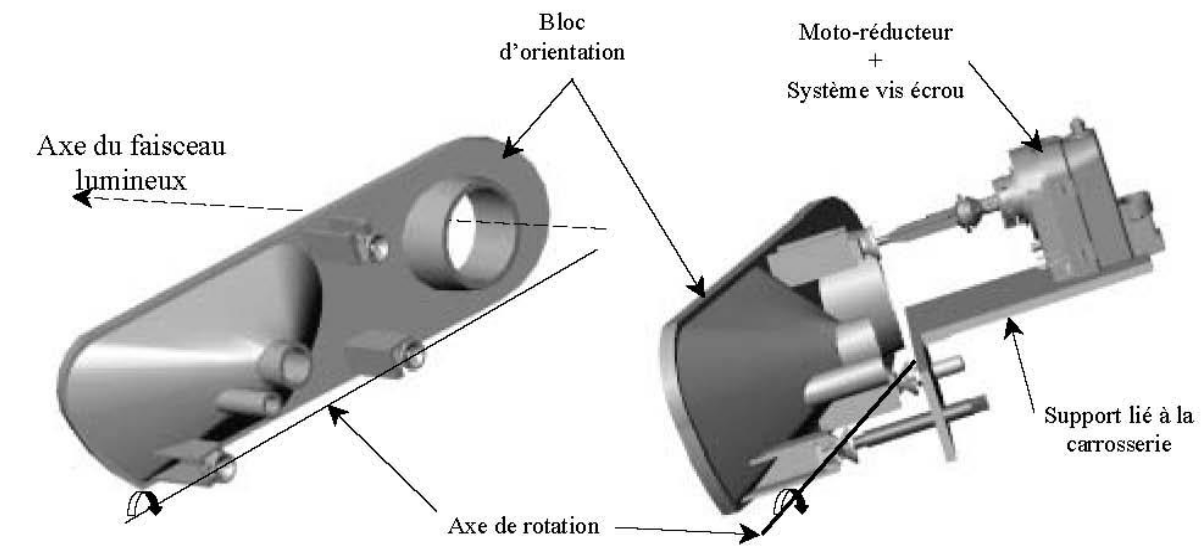
\includegraphics[width=.6\textwidth]{png/image2}
\end{center}

\subsubsection*{Diagrammes SADT niveau A-0, A0 et A3}
\begin{center}
 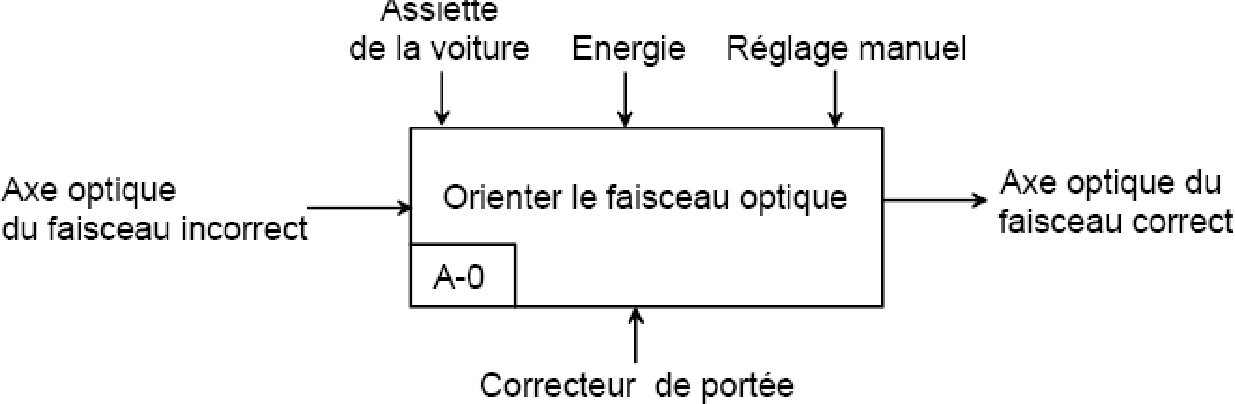
\includegraphics[width=.6\textwidth]{png/image3}
\end{center}

\subsection*{Étude de la chaîne d’action complète}
La chaîne d‘action complète comprend :
\begin{itemize}
 \item l‘ensemble transducteur (\textbf{capteur + amplificateur + calculateur})
qui mesure l‘angle de tangage $\beta$ du véhicule et commande le moteur du
système. L‘ensemble est assimilable à un gain pur : $K_c$;
\item le \textbf{moteur à courant continu} dont la fonction de transfert est
notée $M(p)$;
\item on équipe ce moteur d‘un retour tachymétrique assimilable à un gain pur : 
   $K_{tachy}=0,03 V.rad^{-1}.s$;
\item le \textbf{réducteur de vitesse} dont le rapport de réduction est de 490;
\item l’ensemble \textbf{vis-écrou} (de pas $p = 6mm$) qui transforme la
rotation de l’axe du réducteur en translation de l’axe de sortie. (NB : 1
tour de la vis fait avancer de 1 pas l’écrou);
\item le \textbf{bloc d‘orientation} : l‘angle de correction de portée
$\theta(t)$ étant petit, on peut linéariser la loi entrée-sortie sur le
domaine d‘utilisation ; l‘angle $\theta(t)$ est proportionnel au déplacement
$x(t)$ de la vis.
\end{itemize}

($\theta(t)$ varie entre $\dfrac{-\pi}{20}$ $\dfrac{\pi}{20}$ et pour
$x(t)$ compris entre -15mm et +15mm).

\subparagraph{}
\textit{Refaire, sur votre copie, le diagramme fonctionnel de la chaîne d‘action
ci-dessous, en précisant le nom des constituants dans les blocs, les
informations véhiculées entre les blocs ainsi que leur symbole et leur unité
(les fonctions de transfert ne seront pas déterminées).}
NB : 
\begin{itemize}
 \item l’entrée $B(p)$ est la transformée de Laplace de $\beta(t)$ et la sortie
$\Theta(p)$, la transformée de Laplace de $\theta(t)$;
\item attention, un bloc modélise le passage de la vitesse angulaire $\Omega(p)$
à la position angulaire $\Theta(p)$.
\end{itemize}

\begin{center}
 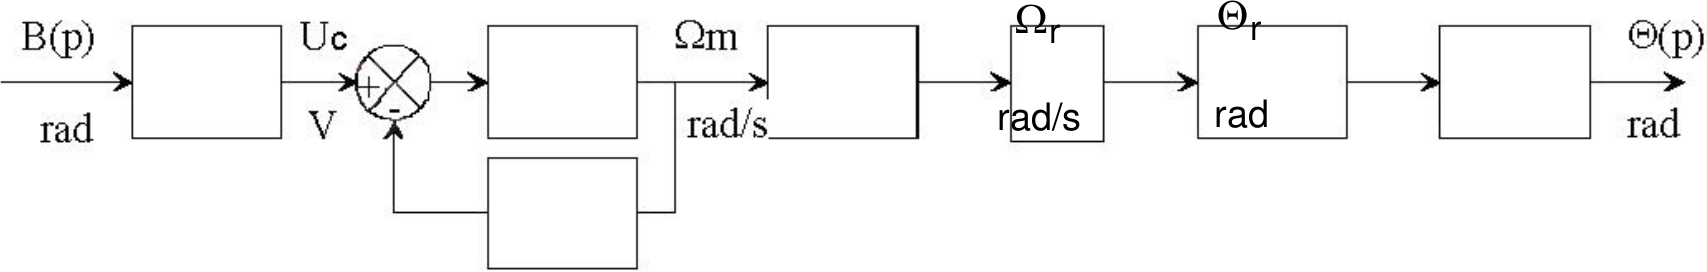
\includegraphics[width=.6\textwidth]{png/image4}
\end{center}

\subparagraph{}
\textit{Refaire, sur votre copie, le diagramme fonctionnel de la chaîne d‘action
ci-dessus, mais cette fois-ci en précisant les fonctions de transfert de chaque
bloc.}

Pour déterminer la fonction de transfert du moteur, $M(p)$, on dispose de sa
réponse indicielle (entrée unitaire) :

\begin{center}
 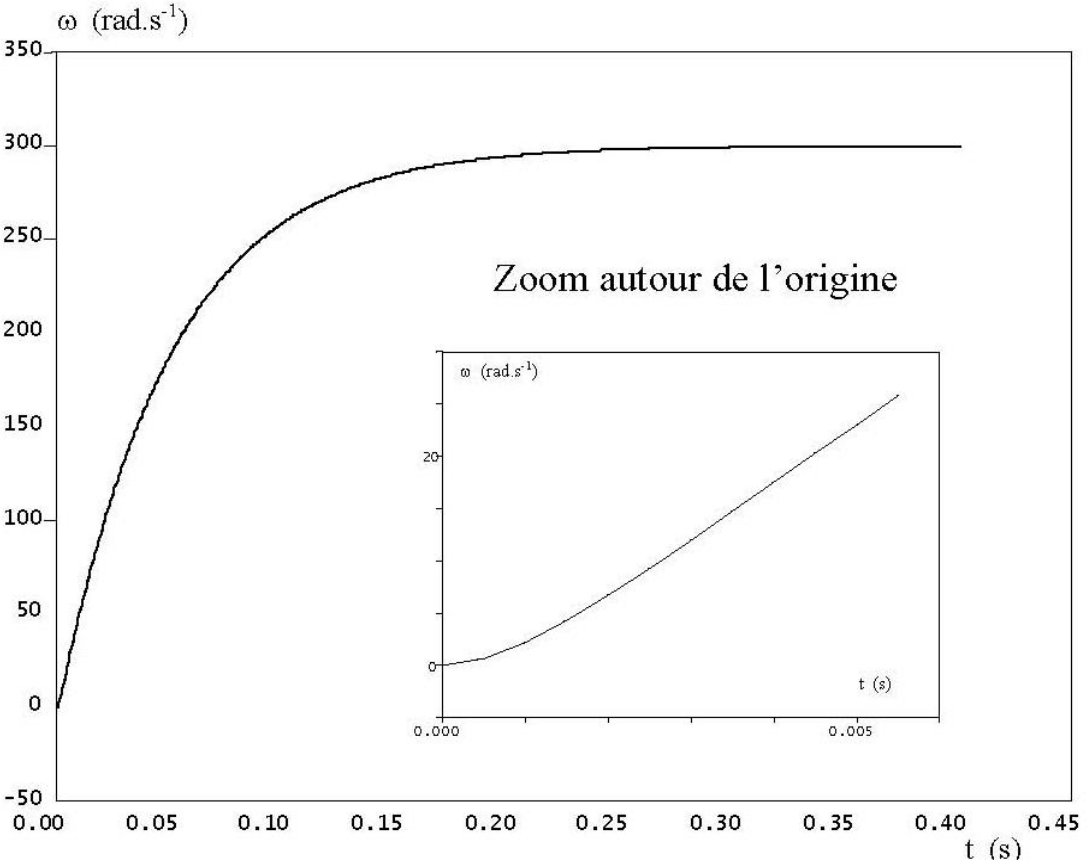
\includegraphics[width=.6\textwidth]{png/image5}
\end{center}

\subparagraph{}
\textit{Quelle est la forme de la fonction de transfert du moteur et pourquoi ?}

\subparagraph{}
\textit{Quelle hypothèse pouvons-nous faire pour modéliser le système par un
système du 1\up{er}
ordre ?
NB : Pour démontrer ce raisonnement, déterminer la réponse temporelle d’un
système
du 2\up{ème} ordre apériodique, puis simplifier cette réponse avec votre
hypothèse et enfin
conclure.
Cette hypothèse vous semble-t-elle justifiée ici au vu de la réponse indicielle.
}

\subparagraph{}
\textit{Identifier $M(p)$ à un 1\up{er} ordre. (Pour cela déterminer les
paramètres caractéristiques sur la courbe).}

\subparagraph{}
\textit{En déduire la fonction de transfert $M'(p)=\dfrac{\Omega_m(p)}{U_c(p)}$
du moteur équipé du retour                                                 
tachymétrique. Quels sont les avantages et les inconvénients de cette boucle de
retour ?}

La fonction de transfert de la chaîne d‘action complète est donnée
approximativement par :
$H(p)=\dfrac{\Theta(p)}{B(p)}=K_c\dfrac{0,003}{\left(1+0,025p \right)p}$    
(Les angles d‘entrée et de sortie sont exprimés en radian).

Le véhicule est brusquement chargé à l‘arrière.

\subparagraph{}
\textit{Tracer, SANS FAIRE DE CALCUL, l‘allure de la loi d‘entrée, puis l‘allure
de la réponse.
Justifier votre tracé. Est-ce satisfaisant ?
}

Pour remédier à ce problème on asservit le système en position en plaçant :
\begin{itemize}
 \item un capteur de position, de gain $K_{pos}$ , qui mesure l‘angle $\theta$,
\item un amplificateur de gain pur $A$.
\end{itemize}

\begin{center}
 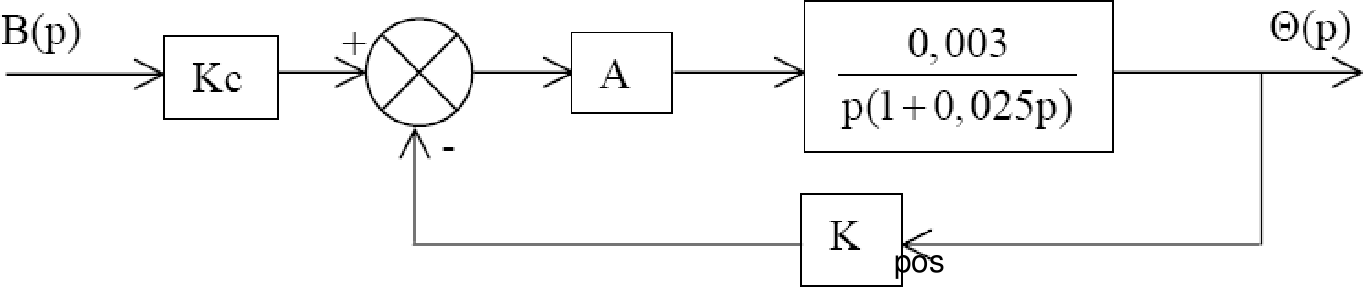
\includegraphics[width=.6\textwidth]{png/image6}
\end{center}

\subparagraph{}
\textit{Déterminer la nouvelle fonction de transfert $\dfrac{\Theta(p)}{B(p)}$
ainsi que ses paramètres caractéristiques.
}

\subparagraph{}
\textit{Expliquer en deux lignes pourquoi le problème a été remédié.}

\subparagraph{}
\textit{À partir de la courbe ci-contre, déterminer la quantité $AK_{pos}$ qui
permet d‘avoir le système le plus rapide. Calculer alors le temps de réponse à
5\% du système.}

\begin{center}
 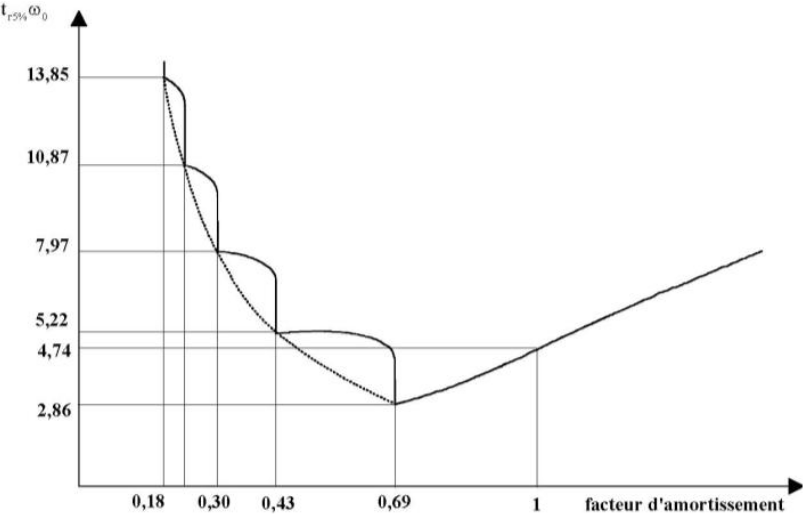
\includegraphics[width=.6\textwidth]{png/image7}
\end{center}


\end{document}
